% Implementation 
\chapter{Implementation}
\label{sec:implement}
This section overviews the implementation and aims to motivate the choice of libraries and frameworks.
We also deliver an in-depth explanation of the implementation of \ac{gdc}, as it is the main focus of our work.
\section{Scope and Limitations}
\label{sec:implement:scope}
Our research is concerned only with graph-level prediction tasks on two types of \acp{gnn}, \ac{gcn} and \ac{gin}.
We implemented both networks as described by~\citet{Kipf2017} and~\citet{Xu2019}, respectively.
We evaluate five different scenarios, among them four different regularization techniques \ac{do}, \ac{ns}, \ac{de}, and \ac{gdc}, and we also train the networks using no regularization.
\Ac{gdc} is implemented as described in \cref{eq:relaxed} since this allows for better time and space complexity, which was also done by~\citet{Hasanzadeh2020}.
We perform our experiments using five datasets from the OGB dataset collection~\cite{Hu2020}, all within the molecular realm.
Two datasets are for classification, and the rest for regression tasks.

\section{Sparse Implementation of Graph Dropout Layers}
% TODO: What is this section about? What is its structure?
This section is concerned with implementing our regularization techniques and explaining how those have been embedded into a convolutional step.
First, we take a look at TensorFlow's gather and scatter operations.
Then, we explain how we use these operations to implement sparse graph convolutions.
For that, an algorithmic description and a text explanation will be presented.
We then explain the implementation of the sparse graph convolutions before we explain how regularization is embedded in a convolutional step.
\label{sec:implement:gnndropout}
% What was used 
\subsection{Gather and Scatter}
\label{sec:implement:gnndropout:gatherscatter}
In \acp{gnn}, communication between nodes is achieved via message passing (see \cref{sec:related:message}).
For messages to be passed along between nodes, we need first to extract and second to pass information on.
For this purpose, we utilize two of TensorFlow's functions, $\mathit{gather}$ and $\mathit{scatter}$~\cite{He2007,Damke2020}.

% Formal definition of gather and scatter 
Formally, the $\mathit{gather}$ operator takes two inputs:
A list $X$ of $n$ row vectors and a list $R$ of $m$ pointers into $X$.
It returns a list $X$ of $m$ row vectors $X[i] = Z[R[i]]$ for $i \in [m]$.
The gather operation in TensorFlow extracts specific elements from a tensor along a given axis.
Given an input tensor and a list of indices, the gather operation selects elements based on the provided indices from the input tensor. Given a tensor representing node features in a graph and a list of node indices, the gather operation extracts the corresponding node features.
The gather operation can extract node features, adjacency information, or other relevant data based on specific graph node indices.

The $\mathit{scatter}_{\Sigma}$ operator can be understood as the opposite of $\mathit{gather}$.
$\mathit{scatter}_{\Sigma}$ takes a list $X$ of $m$ row vectors and a list $R$ of $m$ pointers from the range $[n]$.
It returns a list $Z$ of $n$ row vectors $Z[i] = \sum_{j \in [m] \land R[j] = i} X[j]$ for $i \in [n]$.
The scatter operation in TensorFlow is the inverse of the gather operation.
It updates the elements of an existing tensor based on the provided indices.
Given an input tensor, a list of indices, and a tensor containing values, the scatter operation replaces elements in the input tensor at the specified indices with the corresponding values from the values tensor.
Gather and scatter operations are crucial for tasks involving graph neural networks \acp{gnn} where information aggregation and dissemination across nodes are essential.
Information from nodes or subgraphs is gathered and aggregated for graph classification tasks to represent the entire graph.
\acp{gnn} can use gather operations to pool information from nodes and perform graph-level predictions.

\subsection{Sparse Implementation of Graph Convolutions}
\label{sec:implement:gnndropout:conv}
In our study, the fundamental mechanism for information exchange among nodes in both \acp{gnn} is implemented through the message-passing mechanism via graph convolutions.
\Acp{gnn} capture complex relationships in convolutional steps within graph-structured data.
The detailed algorithm for implementing this message-passing mechanism using graph convolutions is described in Algorithm \ref{algo:sparse_graph_convolution}.
Algorithm \ref{algo:sparse_graph_convolution} outlines the Sparse Graph Convolution operation, where information is efficiently exchanged between nodes utilizing gather and scatter operations.
In this algorithm, the gather operation extracts feature information from neighboring nodes, while the scatter operation aggregates and updates the node representations.
The resulting updated node features are the foundation for subsequent graph convolutional layers.

% Pseudocode / reference lines 
The fundamental operation in our \acp{gnn} is the graph convolution operation, which allows nodes to aggregate and exchange information with their neighboring nodes.
The sparse implementation of graph convolutions can be described algorithmically as follows:
\begin{algorithm}[H]
    \caption{Sparse Graph Convolution using Gather and Scatter}\label{algo:sparse_graph_convolution}
    \begin{algorithmic}[1]
        \Function{$SparseGraphConvolution$}{$X \in \mathbb{R}^{n \times d}, R \in {[n]}^{m \times 2}$}
        \State{$X_{a} \coloneqq \mathit{gather}(Z, R[:,0])$} \label{line:gather1}
        \Comment{Gather Operation: $\mathbb{R}^{n \times d} \times {[n]}^{m} \to \mathbb{R}^{m \times d}$}
        \State{$X_{b} \coloneqq \mathit{gather}(Z, R[:,1])$} \label{line:gather2}
        \State{$X_{\Sigma a} \coloneqq \mathit{scatter}_{\Sigma}(X_{a}, R[:,1])$}  \label{line:scatter1}
        \Comment{Scatter Operation: $\mathbb{R}^{m \times d} \times {[n]}^{m} \to \mathbb{R}^{n \times d}$}
        \State{$X_{\Sigma b} \coloneqq \mathit{scatter}_{\Sigma}(X_{b}, R[:,0])$}  \label{line:scatter2}
        \State{$X_{\text{conv}} \coloneqq \sigma\left(X + X_{\Sigma a} +X_{\Sigma b} \right)$} \label{line:sum}
        \Comment{Result with added self-connections}
        \State{\Return{$X_{\text{conv}}$}} \label{line:res}
        \Comment{Result with added self-connections}
        \EndFunction{}
    \end{algorithmic}
\end{algorithm}
Note that~\cref{algo:sparse_graph_convolution} assumes bidirectional edges.
Hence, the gather and scatter operations are performed twice.
This operation can be efficiently implemented using gather and scatter operations, enabling the network to learn expressive node representations while considering the graph's topology.
In graph convolutions, the gather operation extracts feature information from neighboring nodes.
For each target node $v_{i}$, the gather operation assembles feature vectors from its neighboring nodes in the graph (\cref{line:gather1,line:gather2}).
These gathered features are then scattered into the feature vector of each target $v_{i}$.
The scatter operation aggregates the gathered features by adding them to each target's feature vector.
It takes the computed features and distributes them back to the corresponding nodes in the graph (\cref{line:scatter1,line:scatter2}).
This step ensures that the updated node representations, enriched with information from neighboring nodes, are propagated throughout the graph.

Lastly, the feature vector of the node itself is added, forming the basis for computation in the subsequent convolutional layer (\cref{line:sum}).
By selecting and aggregating features from neighboring nodes using the gather and scatter operations, the model captures the local neighborhood information critical for graph-based tasks.
With each convolution, one additional neighborhood can be captured.
This way, both local and global patterns are captured.

% Implementation of Regularization techniques - general idea 
% The most important one 
\subsection{Adding Dropout to Sparse Graph Convolutions}
\label{sec:implement:gnndropout:dropout}
Four of our regularization techniques, described in \cref{sec:related:pred:regularization}, have been integrated into this gather/scatter-based graph convolution.
We implement those techniques using a unified framework.
We are using just two parameters, \textit{row-wise?} and \textit{gather-first?}.
We describe all four dropout techniques in \cref{sec:related:pred:regularization}.

The \textit{row-wise?} parameter tells us if the dropping is done for entire rows or just for some values in the rows of a feature matrix.
The feature matrix $X$, where each row represents a node, and each entry in such a row represents a feature of the node.
This vector is masked when we perform \ac{do} or \ac{ns}.
Each row of the gathered matrices $X_a$ and $X_b$ contains the feature vector of the start node of an edge.
We perform \ac{de} and \ac{gdc} by masking those gathered matrices.
Masking is implemented as element-wise multiplication with the corresponding vectors.

So, the whole node is dropped when \textit{row-wise?} is true.
This is the case for \acf{ns} and for \acf{de}. \Ac{ns} removes the whole node, along with every feature of this node, and \ac{de} is concerned with dropping edges, i.e., connections to the entire node, not only to some of the features.
So, this type of dropout is also performed row-wise.
\Acf{do} drops just some features of a gíven node, so the \textit{row-wise?} parameter is set to false.
This is also the case for \acp{gdc} as it draws random masks, i.e., performs drops for each channel independently.

The \textit{gather-first?} parameter tells us whether the mask is applied before or after we gather values.
When \textit{gather-first?} is set to true, we gather the values and then apply the mask, meaning that the mask is applied to $X_{a}$ and $X_b$.
This is the case for \ac{de} and \ac{gdc}.
When \textit{gather-first?} is set to false, which is the case for \ac{do} and \ac{ns}, we apply the mask and then gather the values.
That means the mask is applied directly to the $X \in \mathbb{R}^{n \times d}$ before we gather values in \cref{line:gather1}.

To sum up, \textit{gather-first?} is the parameter that regulates which matrix the randomly drawn mask is applied, and \textit{row-wise?} determines if the ``random drop'' is valid for the whole row.
The permutations of those two parameters result in four of our regularization techniques~\cref{table:dropout}.
The different types of regularization are all performed in each gather/scatter-based convolutional step by masking some values from the feature vector $X$ or $X_a$ and $X_b$.

We implement regularization by integrating the masking of values in each gather/scatter-based convolutional step.
\begin{center}
    \begin{tabular}{lll}
        \toprule
        \textbf{Regularization} & \textbf{row-wise?} & \textbf{gather-first?} \\
        \midrule
        \acf{do}                & false              & false                  \\
        \acf{de}                & true               & true                   \\
        \acf{ns}                & true               & false                  \\
        \acf{gdc}               & false              & true                   \\

        \bottomrule
    \end{tabular}
    \label{table:dropout}
\end{center}

Since our research is first and foremost focused on validating the results of mainly \ac{gcn}, we aim to elicit a better understanding of this technique.
We look at the two proposed variants of \ac{gdc} and provide an intuition for both.
The second, more relaxed version of \ac{gdc}, as described in~\cref{fig:implementaion:GDC-eq5} was implemented for our research, as it allowed for better time and space complexity and was also the one that was originally evaluated by \citep{Hasanzadeh2020}.

As stated previously in \cref{sec:related:pred:regularization:gdc}, this version of \ac{gdc} allows drawing different random masks for each channel and edge independently, giving more flexibility and increasing the time and space complexity.
\begin{equation}
    \begin{aligned}
        H^{(l+1)}[:,j] & = \sigma \left(\sum_{i=1}^{f_{l}}\mathfrak{R}\left(A \odot Z_{i,j}^{(l)}\right)H^{(l)}[:,i]W^{(l)}[i,j]\right) \\
        \text{for } j  & = 1,..., f_{l+1}
    \end{aligned}\label{eq:implementaion:GDC-eq4}
\end{equation}
\begin{figure}[ht]
    \centering
    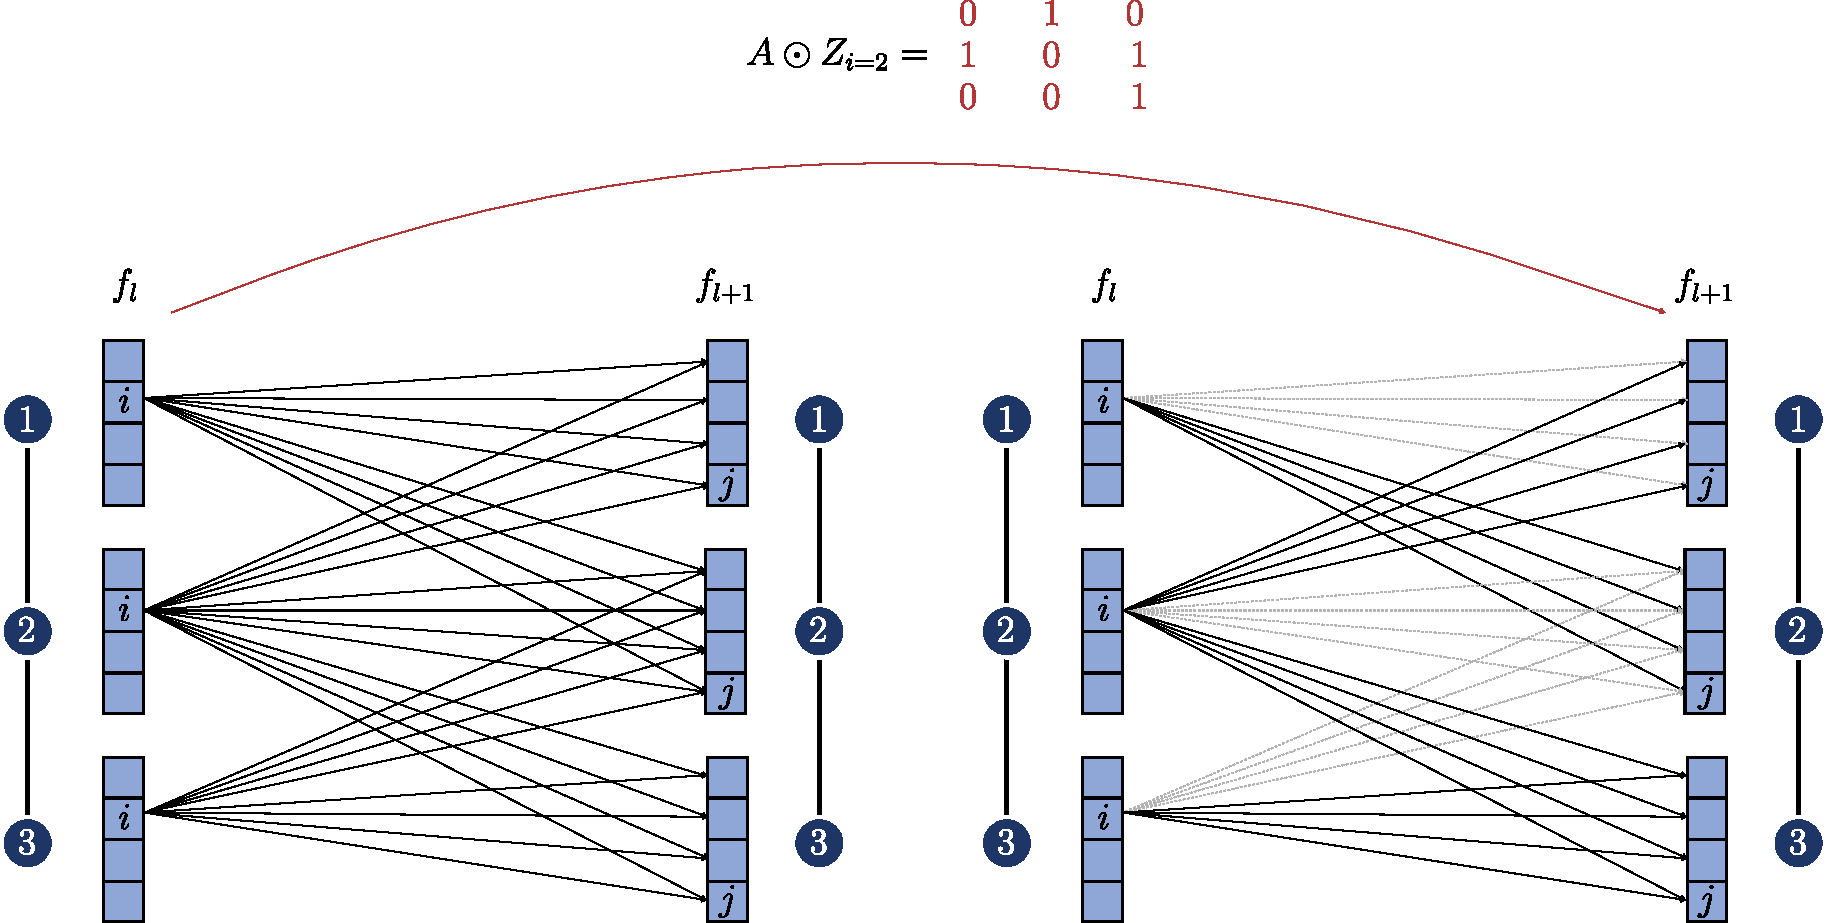
\includegraphics[width= 0.90\linewidth]{gfx/implementation/GDC-eq5.pdf}
    \caption{Originally proposed \ac{gdc}Note: self connection are assumed}\label{fig:implementaion:GDC-eq5}
\end{figure}
% Description and Intuition for GDC-eq4
Here, we calculate the new feature matrix $H^{(l+1)}$ by stacking the column vectors of each iteration. One can think of the calculations that are being performed as a $4$-dimensional matrix with the dimensions $n\times n\times f_{l}\times f_{l+1}$

To understand what is being done, we can look at what is being performed when calculating one column of the resulting matrix. First, a random mask is applied to the connection from the $i$-th to the $j$-th node. Regarding node features communicating with each other, we look at the edge between the $i$-th and $j$-th features between connected nodes. By applying the random mask, we drop those connections selectively. Because we sample the random binary mask $Z$ $f_{l+1}$ times, one time for every feature in the $l+1$-th iteration, we differentiate between the connection $i \rightarrow j$ between two nodes and the connection $j \rightarrow i$ between the same two nodes. Thus, the same edge can be dropped as a connection and remain as a connection in the opposite direction. The masked adjacency is then multiplied by the corresponding column and weight.
One may think of it as performing a random sampling across each channel since in each iteration from $i=1$ to $f_{l+1}$, we perform multiplication with the $i-th$ column of $H$.

As for the implementation of \ac{gdc}, we decided to implement the less complex version, as shown below, since this implementation reduces the runtime completely and is also the one that was originally implemented for testing the efficacy of \ac{gdc}.

\begin{align}
    H^{(l+1)} = \sigma(\sum_{i= 1}^{f_{l}}\mathfrak{N}(A \odot Z_{i}^{(l)})H^{(l)}[:,i] W^{(l)}[i,:]) \label{eq:relaxed}
\end{align}
\begin{figure}[ht]
    \centering
    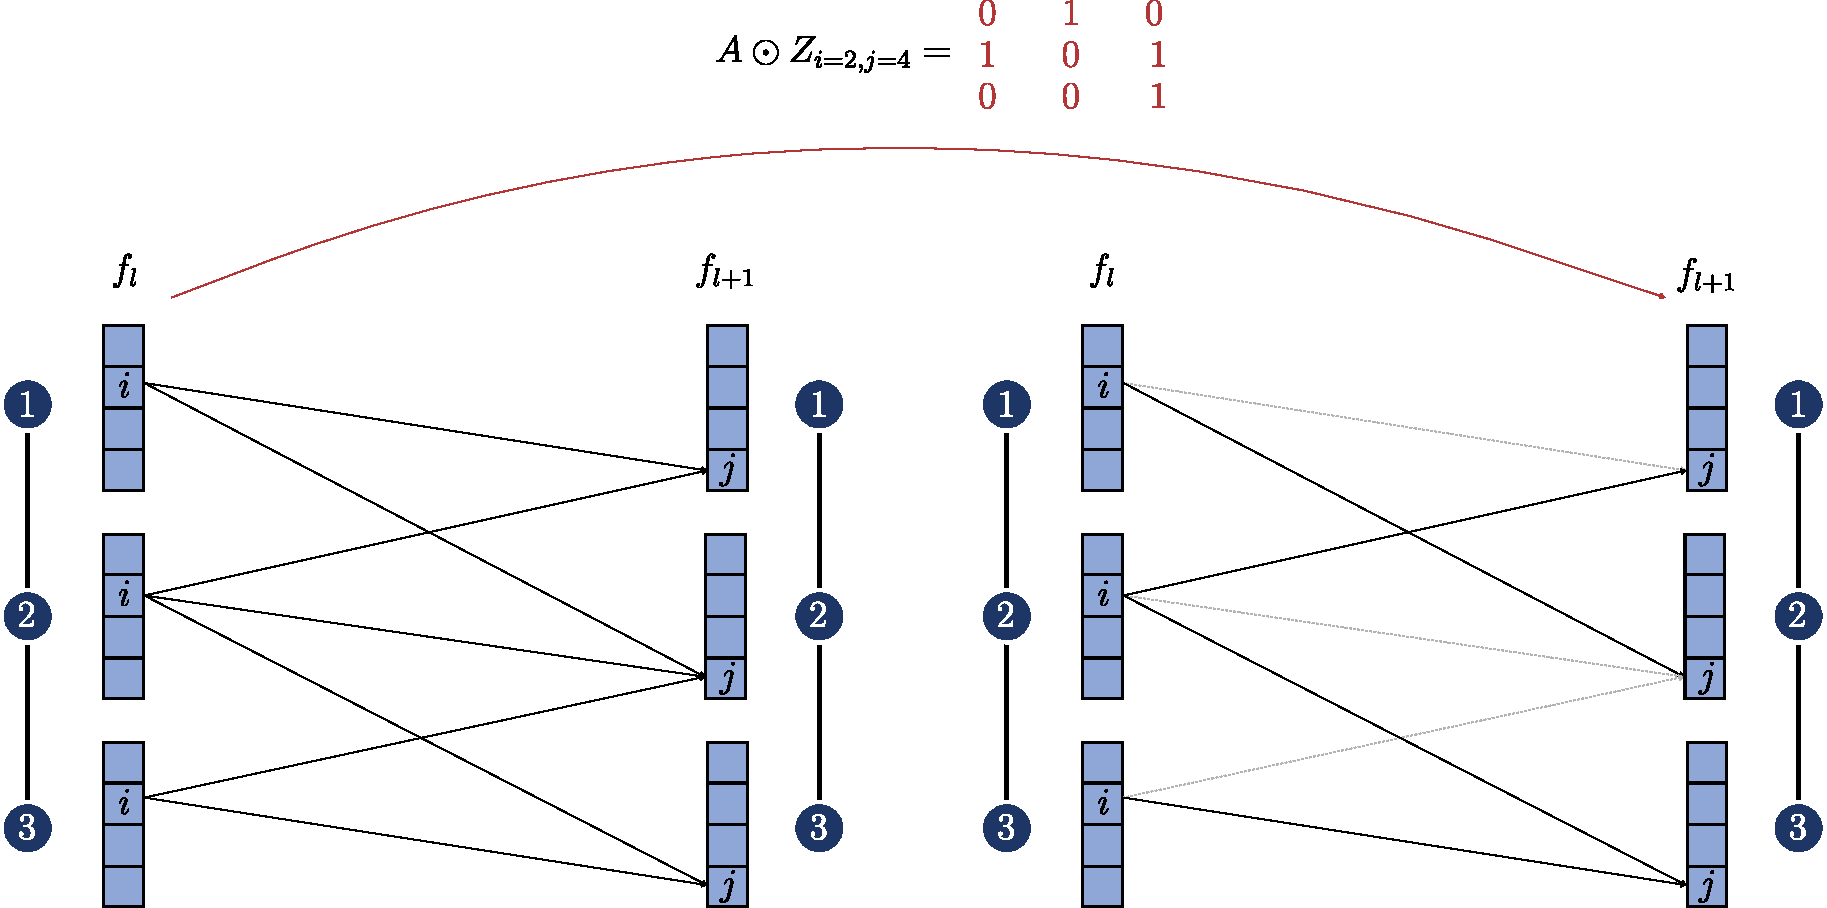
\includegraphics[width= 0.90\linewidth]{gfx/implementation/GDC-eq4.pdf}
    \caption{\Ac{gdc}Note: self connection are assumed}\label{fig:implementaion:GDC-eq4}
\end{figure}
Here, we compute the new feature matrix in one go instead of doing $f_{l}$ iterations for all $f_{l}$ columns.


\section{Choice of Libraries and Frameworks}
\label{sec:implement:frameworks}
Below, we briefly overview the datasets and frameworks used and motivate the choice.
% \subsection{Datasets}
% \label{sec:implement:frameworks: datasets}
% Datasets - OGB 
Even though machine learning on graph-structured data is carried out in many areas and has many interesting use cases ranging from social networks to molecular graphs, manifolds, and source code~\cite{Hu2020},
there is no unified framework for working with graph-structured data.
Furthermore, commonly used datasets and evaluation procedures suffer from multiple issues that negatively affect the quality of predictions and the reliability of evaluations of models.
Machine learning algorithms rely heavily on data. For a \ac{gnn} to be able to make accurate predictions, there is a need for a sufficient amount of properly prepared training data. Standardized splitting and evaluation methods are needed to compare different models against each other.

% Problems overview 
Today, most of the frequently used graph datasets are extremely small compared to graphs found in real applications.
The same datasets, such as Cora, CiteSeer, and PubMed, are used repeatedly to train different models, leading to poor scalability in most cases. Small datasets also make it hard to rigorously evaluate data-hungry models, such as \acfp{gnn}.
The performance of a \ac{gnn} on these datasets is often unstable and nearly statistically identical due to the small number of samples the models are trained and evaluated on~\cite{Kipf2017,Xu2019, Hu2020}.

% OGB benefits  
\textbf{\Ac{ogb}} offers a wide range of different-sized graph datasets from different domains for a variety of varying classification tasks and provides a unified pipeline for working with the datasets in \ac{ml} tasks.
The unified experimental protocol with standardized dataset splits, evaluation metrics, and cross-validation protocols makes it easy to compare performance reported across several studies~\cite{Hu2020}.

% Overview of standardized pipeline 
Working with \ac{ogb} consists of following steps:

\begin{enumerate}
    \item \Ac{ogb} provides realistic, different-scaled graph benchmark datasets that cover different prediction tasks from diverse applications.
    \item Dataset processing and splitting is fully automated. \Ac{ogb} data loaders automatically download and process graphs and further split the datasets in a standardized manner.
          This is compatible with multiple libraries and provides a library-agnostic option.
    \item This step includes developing an \ac{ml} model to train on the \ac{ogb} datasets.
    \item  \Ac{ogb} evaluates the model in a dataset-dependent manner and outputs the model performance appropriate for the task at hand.
    \item \Ac{ogb} provides public leaderboards to keep track of recent advances.
\end{enumerate}

\begin{figure}[H]
    \centering
    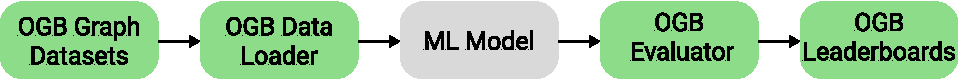
\includegraphics[width= 0.90\linewidth]{gfx/implementation/OGB_pipeline}
    \caption{\textbf{Overview of the standardized OGB pipeline} adapted from \cite{Hu2020}}\label{fig:implement:pipeline}
\end{figure}

%  3.3 Choice of Libraries and Frameworks (mention TensorFlow and NetworkX)
For machine learning tasks, TensorFlow, a powerful and versatile open-source machine learning framework, was a fundamental tool for developing and training intricate machine learning models.
TensorFlow's extensive set of libraries and tools simplifies the process of building, training, and deploying machine learning models, making it a preferred choice.
The framework's adaptability to many tasks, from image recognition to natural language processing, underscores its universal applicability, positioning it at the forefront of modern machine learning research.
In addition to TensorFlow, this study leveraged NetworkX, a Python package designed to create, manipulate, and analyze complex networks. NetworkX was used as a tool for graph representation.
